\documentclass[aspectratio=169]{beamer}
\usepackage[utf8]{inputenc}
%\usepackage[width=160,height=90]{geometry}
\usepackage{graphicx}
\usepackage{multicol}
\usepackage{hyperref}

\renewcommand{\sfdefault}{phv}

\usetheme{Montpellier}

\definecolor{adngreen}{RGB}{51,122,183} %d9534f %337ab7  0,167,127 | 51,122,183 | 235, 83, 79
\setbeamercolor{title}{fg=white}

\setbeamercolor{frametitle}{fg=white}
\setbeamercolor{structure}{bg=adngreen,fg=adngreen}
\setbeamercolor{subsection in sidebar}{fg=white}





\title{\textbf{M183} \\Indirect Direct Object Reference}
\author{Timo Bonomelli, Patrick Günthard}



\AtBeginSection[]
{
  \begin{frame}
    \frametitle{Table of Contents}
    \tableofcontents[currentsection]
  \end{frame}
}

\begin{document}

\frame{\titlepage}

%\begin{frame}
%  \frametitle{Table of Contents}
%  \tableofcontents
%\end{frame}
\section{Vulnerability}


\begin{frame}
  \frametitle{What is \textit{Insecure Direct Object References}}
  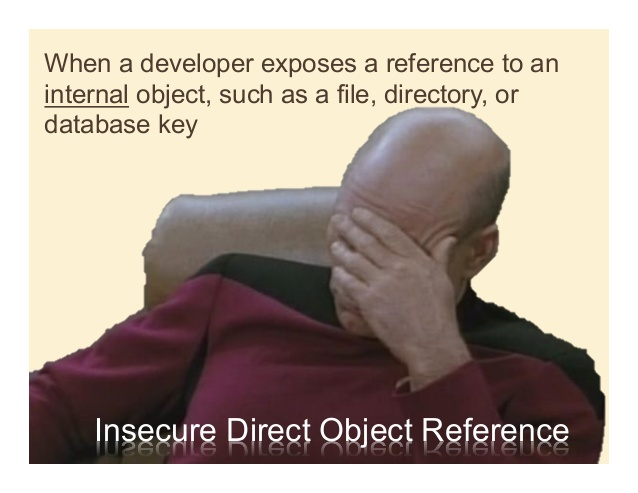
\includegraphics[width=8cm]{meme}
\end{frame}

\subsection{Threats}
 
\begin{frame}
  \frametitle{Threats}
  \begin{itemize}
  \item \textbf{Threat Agents:} Any user who has only partial access to certain type of system data
  \item \textbf{Attacker's Approach:} Attacker, an authorized system user, simply changes a parameter value that directly refers to a system object to another object the user isn't authorized to use
  \item \textbf{Security Weakness:} Applications don’t always verify the user is authorized for target objects
  \end{itemize}
\end{frame}

\subsection{Example}

\begin{frame}[fragile]
  \label{examplecode}
  \frametitle{Example: Code}
  \textit{Example Website:}\\\tiny
\dots
\begin{verbatim}
String query = "SELECT * FROM accts WHERE account = ?";
PreparedStatement pstmt = connection.prepareStatement(query , ... );
pstmt.setString( 1, request.getParameter("acct"));
ResultSet results = pstmt.executeQuery();
\end{verbatim}
\dots\\
\tiny\textit{2010 OWASP - CC-BY-SA}
\normalsize
\end{frame}


\begin{frame}
  \frametitle{Example: Attack}
  \begin{multicols}{2}
   \LARGE{Normal behavior}\\\normalsize Example URL: \small\texttt{http://example.com/app/ accountInfo?acct=\textit{myacct}}\\
   \normalsize{Result:}\\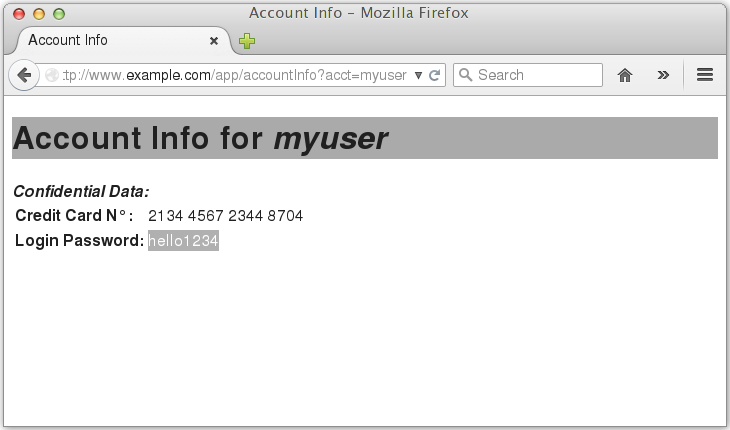
\includegraphics[width=5cm]{example_web_s1}\\
   \LARGE{Attack behavior}\\\normalsize Example URL: \small\texttt{http://example.com/app/ accountInfo?acct=\textit{notmyacct}}\\
   \normalsize{Result:}\\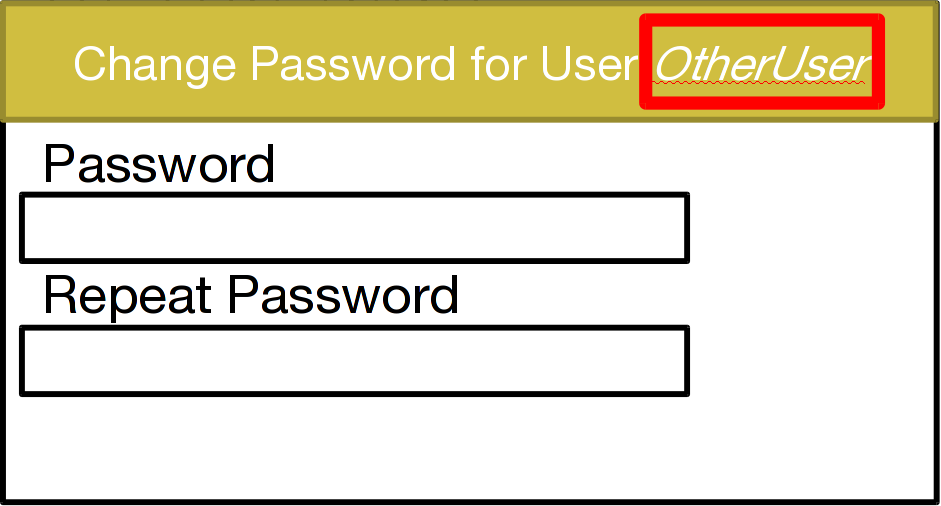
\includegraphics[width=5cm]{example_web_s2}\\
  \end{multicols}
\end{frame}

\begin{frame}
  \frametitle{Example: Attack}
  This URL:\\ \texttt{app/accountInfo?acct=\textit{myacct'; DROP accts; }} (\ref{examplecode})
\end{frame}


\section{How to prevent an Attack}

\subsection{Session Based}

\begin{frame}
  \frametitle{Session}
  \begin{itemize}
    \item No \textit{Direct Object Reference} has to be sent to the client, the references can be saved on the session
    \item In the case references are needed, they can differ from the server side data (i.e. database) an can be remapped on the server
  \end{itemize}
\end{frame}

\subsection{Authentication on every access}

\begin{frame}
  \frametitle{Authentication}
  \begin{itemize}
    \item Every access is checked if the user is authorized to do that. Example: A random token can be created for each user which then is checked every time the user accesses the page
  \end{itemize}
\end{frame}

\subsection{Solutions and Problems}

\begin{frame}
  \frametitle{Solutions and Problems}
\tiny
  \begin{tabular}{|l|p{4cm}|p{4cm}|}
    \hline
    & \textbf{Advantage} & \textbf{Disadvantage} \\\hline
    \textbf{Session Based} & Only one authorization has to be done, access data for Database etc. is saved on the server and is not accessible by the attacker & A session uses a lot of memory for each user. For applications with a high number of users, a session for each client is not possible i.e. a non-session solution has to be implemented \\\hline
    \textbf{Authentication} & No Session is needed i.e. less memory is used and more users can access the application & Authorization is needed every time the user accesses data which is more complex to implement\\\hline
  \end{tabular}
\end{frame}


\section{Summary}

\begin{frame}
  \frametitle{Summary}
  \begin{itemize}
    \item Serious Issue
    \item Easily preventable
    \item Several fixing solutions
  \end{itemize}
\end{frame}

\begin{frame}
  \frametitle{End}
  Sources:\\
  \begin{itemize}
    \item \href{https://www.owasp.org/index.php/Top_10_2010-A4-Insecure_Direct_Object_References}{OWASP: 2010-A4-Insecure Direct Object References}
    \item \href{https://en.wikipedia.org/wiki/HDIV}{Wikipedia: HDIV}
  \end{itemize}


\includegraphics[width=1cm]{cc.png}
  
\end{frame}

\end{document}